\documentclass[18pt]{article}

\usepackage[utf8]{inputenc}
\usepackage[T1]{fontenc}
\usepackage{ragged2e}
\usepackage{caladea}
\usepackage{graphicx}
\usepackage{longtable}
\usepackage{wrapfig}
\usepackage{rotating}
\usepackage{epigraph}
\usepackage[normalem]{ulem}
\usepackage{hyperref}
\usepackage{amsmath}
\usepackage{amssymb}
\usepackage{capt-of}
\usepackage{fancyhdr}

\title{
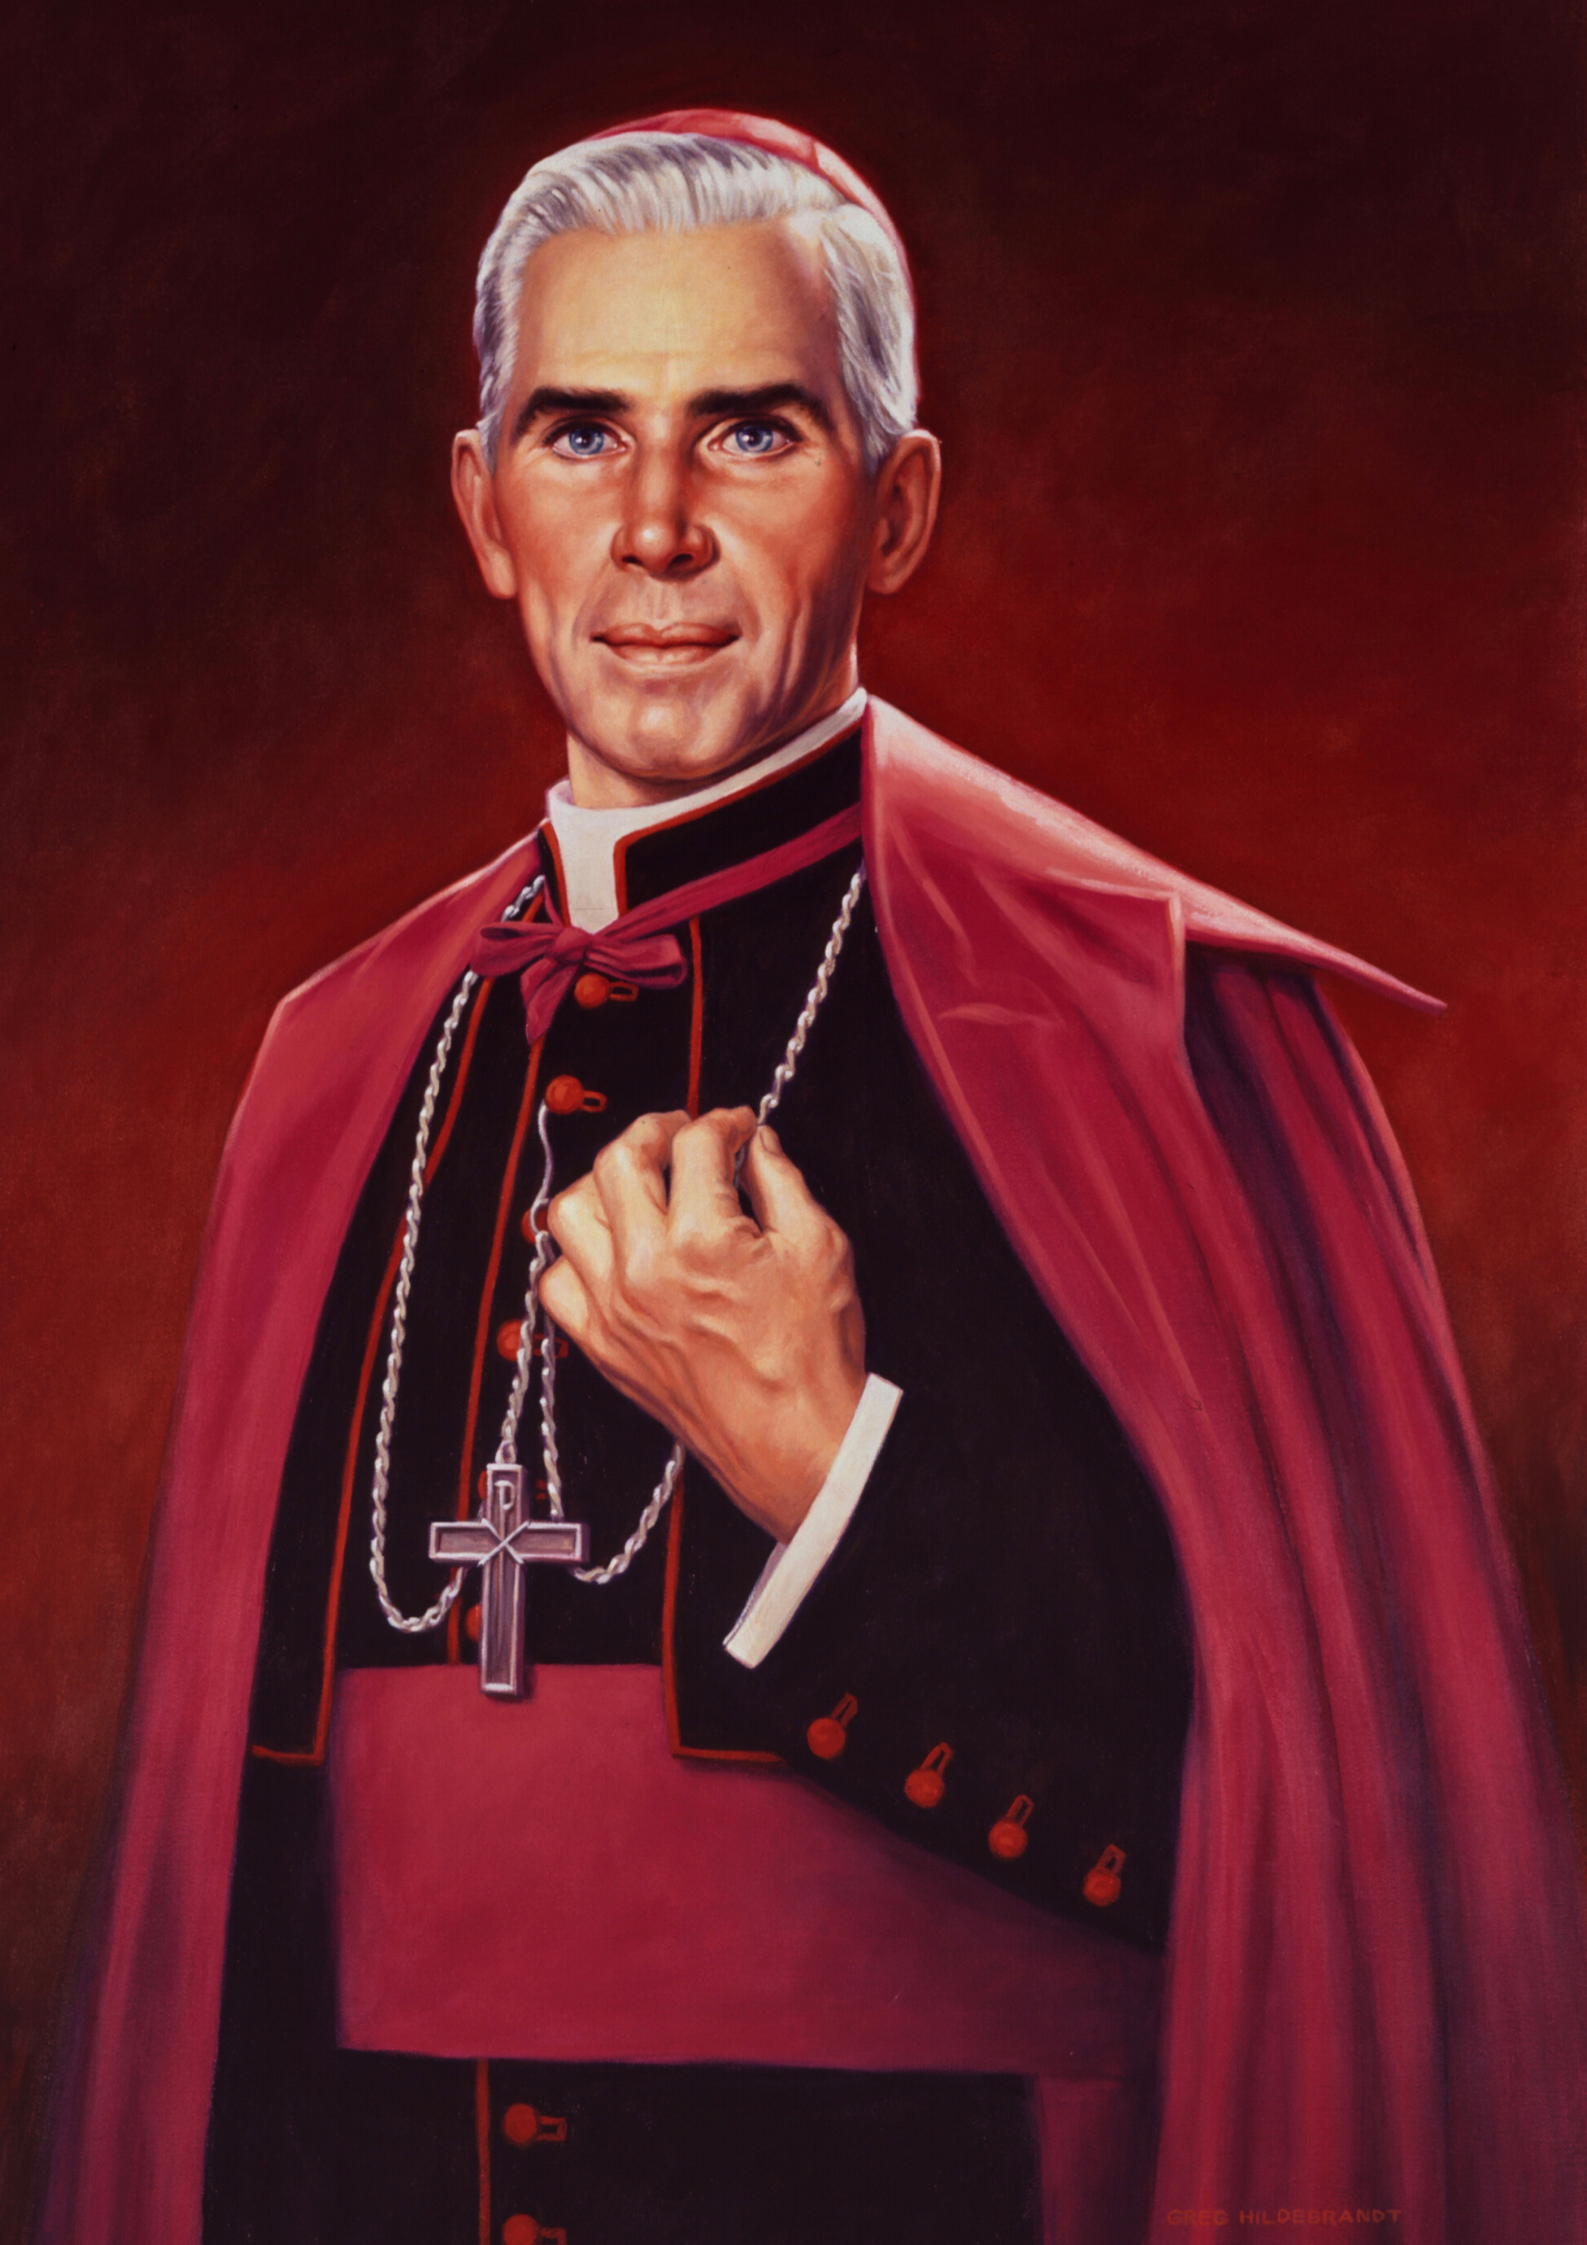
\includegraphics[scale=.75, trim={10cm, 0, 10cm, 0}]{./assets/imagem.jpg}
\par
Novena ao Beato Iván Merz
}

\date{Data de Início: 01/05 \quad Data Litúrgica: 10/05}

% Comando para fazer "Sumário" não aparecer no Sumário.
\renewcommand{\contentsname}{Sumário}

\begin{document}

\thispagestyle{empty} %zera a primeira página

\maketitle

\begin{center}
Visite-nos no Telegram: \url{https://t.me/CotidieNovena}
\end{center}

\pagestyle{fancy}
\fancyhf{} % clear existing header/footer entries
\fancyfoot[LO, CE]{
\includegraphics[scale=0.2]{./assets/cross.png} Beato Iván Merz, rogai por nós!
}
\fancyfoot[R]{\thepage}

\newpage

\tableofcontents

\newpage

%%%%%%%%%%%%%%%%%%%%%%%%%%%%%%%%%%%%% História %%%%%%%%%%%%%%%%%%%%%%%%%%%%%%%%%%%%%%%%%%%

\begin{justify}
\begin{center}
\section{História}\label{sec:História}
\end{center}

Iván Merz nasceu em 16 de dezembro de 1896, em Banja Luka, na Bósnia, então parte do Império Austro-Húngaro. Desde jovem, destacou-se por sua inteligência e profunda sensibilidade religiosa. Durante a Primeira Guerra Mundial, serviu como oficial do exército, experiência que marcou profundamente sua vida espiritual. Após a guerra, dedicou-se aos estudos universitários em Viena e Paris, onde aprofundou seu conhecimento sobre a liturgia e a doutrina católica.

De volta à Croácia, Iván tornou-se um grande apóstolo entre a juventude, promovendo o Movimento Litúrgico e incentivando a participação ativa dos leigos na vida da Igreja. Fundou e liderou a associação "A Cruzada dos Jovens Croatas", inspirando muitos a buscar a santidade no cotidiano. Sua vida foi marcada por intensa oração, amor à Eucaristia e dedicação à formação cristã da juventude.

Iván Merz faleceu em 10 de maio de 1928, aos 31 anos, após uma breve enfermidade, oferecendo seus sofrimentos pela Igreja e pela juventude. Foi beatificado por São João Paulo II em 22 de junho de 2003. O Beato Iván Merz é modelo de santidade leiga, zelo apostólico e amor à liturgia.

\vfill

\begin{center}
\href{https://www.vatican.va/news_services/liturgy/saints/ns_lit_doc_20030622_merz_po.html}{Fonte: Vatican News}
\end{center}
\end{justify}

%%%%%%%%%%%%%%%%%%%%%%%%%%%%%%%%%%%%% Orações %%%%%%%%%%%%%%%%%%%%%%%%%%%%%%%%%%%%%%%%%%%

\newpage

\begin{center}
\section{Orações}\label{sec:Orações}
\textit{Em nome do Pai, e do Filho, e do Espírito Santo. Amém.}
\end{center}

\subsection*{Oração Inicial}\label{sec:Oração_Inicial}
Deus eterno e todo-poderoso, que destes ao Beato Iván Merz a graça de buscar a santidade no cotidiano, de amar profundamente a Eucaristia e de servir com ardor à juventude, concedei-me, por sua intercessão, a graça de viver com fidelidade a minha vocação cristã e de crescer no amor à vossa Igreja. Amém.

\subsection*{Ato de Contrição}\label{sec:Ato_de_Contrição}
Meu Deus, eu me arrependo de todo o coração de Vos ter ofendido, porque sois infinitamente bom e digno de ser amado sobre todas as coisas. Proponho firmemente, com o auxílio de Vossa graça, não mais pecar. Amém.

\subsection*{Oração Final}\label{sec:Oração_Final}
Beato Iván Merz, que fostes exemplo de fé, esperança e caridade, ajudai-me a buscar a santidade em minha vida diária. Intercedei junto a Deus para que eu persevere no caminho do bem, amando a Igreja e servindo aos irmãos com alegria. Por Cristo, Nosso Senhor. Amém.

\textbf{\textit{Rezar três Pai-Nossos, uma Ave-Maria e um Glória ao Pai em honra à Santíssima Trindade.}}

\textbf{Em nome do Pai, e do Filho, e do Espírito Santo. Amém.}

\vfill

%%%%%%%%%%%%%%%%%%%%%%%%%%%%%%%%%%%%% Orações de Cada Dia %%%%%%%%%%%%%%%%%%%%%%%%%%%%%%%%%%%%%%%%%%%

\subsection*{Orações de Cada Dia}

\subsection*{Primeiro Dia}
\textbf{\textit{\nameref{sec:Oração_Inicial}}}

Beato Iván Merz, que desde jovem buscaste a verdade e a santidade, alcançai-me a graça de um coração aberto à vontade de Deus e sedento de Sua presença.

\textbf{\textit{\nameref{sec:Ato_de_Contrição} e \nameref{sec:Oração_Final}}}

\subsection*{Segundo Dia}
\textbf{\textit{\nameref{sec:Oração_Inicial}}}

Beato Iván Merz, apóstolo da juventude, ajudai-me a ser testemunha fiel de Cristo entre meus irmãos, especialmente entre os jovens.

\textbf{\textit{\nameref{sec:Ato_de_Contrição} e \nameref{sec:Oração_Final}}}

\subsection*{Terceiro Dia}
\textbf{\textit{\nameref{sec:Oração_Inicial}}}

Beato Iván Merz, amante da Eucaristia, ensinai-me a valorizar a Santa Missa e a adoração ao Santíssimo Sacramento, fonte de toda santidade.

\textbf{\textit{\nameref{sec:Ato_de_Contrição} e \nameref{sec:Oração_Final}}}

\subsection*{Quarto Dia}
\textbf{\textit{\nameref{sec:Oração_Inicial}}}

Beato Iván Merz, promotor da liturgia, fazei que eu compreenda e ame cada vez mais a riqueza dos ritos da Igreja, vivendo-os com fervor.

\textbf{\textit{\nameref{sec:Ato_de_Contrição} e \nameref{sec:Oração_Final}}}

\subsection*{Quinto Dia}
\textbf{\textit{\nameref{sec:Oração_Inicial}}}

Beato Iván Merz, que soubeste unir estudo e oração, ajudai-me a buscar a verdade e a sabedoria, colocando tudo a serviço do Reino de Deus.

\textbf{\textit{\nameref{sec:Ato_de_Contrição} e \nameref{sec:Oração_Final}}}

\subsection*{Sexto Dia}
\textbf{\textit{\nameref{sec:Oração_Inicial}}}

Beato Iván Merz, que ofereceste teus sofrimentos pela Igreja, ensinai-me a aceitar com amor as dificuldades da vida, unindo-as ao sacrifício de Cristo.

\textbf{\textit{\nameref{sec:Ato_de_Contrição} e \nameref{sec:Oração_Final}}}

\subsection*{Sétimo Dia}
\textbf{\textit{\nameref{sec:Oração_Inicial}}}

Beato Iván Merz, fiel leigo, concedei-me a graça de viver com alegria e responsabilidade minha missão na Igreja e no mundo.

\textbf{\textit{\nameref{sec:Ato_de_Contrição} e \nameref{sec:Oração_Final}}}

\subsection*{Oitavo Dia}
\textbf{\textit{\nameref{sec:Oração_Inicial}}}

Beato Iván Merz, intercessor junto a Deus, peço-te que apresentes ao Senhor minhas intenções e necessidades, especialmente: (mencionar graça desejada).

\textbf{\textit{\nameref{sec:Ato_de_Contrição} e \nameref{sec:Oração_Final}}}

\subsection*{Nono Dia}
\textbf{\textit{\nameref{sec:Oração_Inicial}}}

Beato Iván Merz, modelo de santidade, alcançai-me a perseverança final e a graça de, um dia, contemplar a Deus face a face no Céu.

\textbf{\textit{\nameref{sec:Ato_de_Contrição} e \nameref{sec:Oração_Final}}}

\centering

\vfill

\subsection*{Créditos:}
\href{https://oracoes.pt/novena-ao-beato-ivan-merz/}{Orações.PT}

\end{document}
